\documentclass[a4paper, 12pt]{article}
\usepackage[english]{babel}
\usepackage[ansinew]{inputenc}
\usepackage{natbib}
\usepackage{graphicx}
\usepackage{listings, lstautogobble}
\usepackage[usenames,dvipsnames]{color}
\usepackage{float}
\usepackage{caption}
\usepackage{subcaption}
\usepackage{wrapfig}
\usepackage{fancyhdr}
\usepackage{amsmath}
\usepackage{algpseudocode}

\pagestyle{headings}


\definecolor{codegray}{gray}{0.92}
\newcommand{\code}[1]{\colorbox{codegray}{\texttt{#1}}}

\lstset{ %
backgroundcolor=\color{codegray},   % choose the background color; you must add \usepackage{color} or \usepackage{xcolor}
basicstyle=\footnotesize,        % the size of the fonts that are used for the code
breakatwhitespace=false,         % sets if automatic breaks should only happen at whitespace
breaklines=true,                 % sets automatic line breaking
captionpos=b,                    % sets the caption-position to bottom
commentstyle=\color{OliveGreen},      % comment style
deletekeywords={...},            % if you want to delete keywords from the given language
escapeinside={\%*}{*)},          % if you want to add LaTeX within your code
extendedchars=true,              % lets you use non-ASCII characters; for 8-bits encodings only, does not work with UTF-8
frame=single,                    % adds a frame around the code
keepspaces=true,                 % keeps spaces in text, useful for keeping indentation of code (possibly needs columns=flexible)
keywordstyle=\color{blue},       % keyword style
language=Octave,                 % the language of the code
morekeywords={*,...},            % if you want to add more keywords to the set
numbers=left,                    % where to put the line-numbers; possible values are (none, left, right)
numbersep=5pt,                   % how far the line-numbers are from the code
numberstyle=\tiny\color{black},  % the style that is used for the line-numbers
rulecolor=\color{black},         % if not set, the frame-color may be changed on line-breaks within not-black text (e.g. comments (green here))
showspaces=false,                % show spaces everywhere adding particular underscores; it overrides 'showstringspaces'
showstringspaces=false,          % underline spaces within strings only
showtabs=false,                  % show tabs within strings adding particular underscores
stepnumber=1,                    % the step between two line-numbers. If it's
stringstyle=\color{mauve},       % string literal style
tabsize=2,                       % sets default tabsize to 2 spaces
title=\lstname                   % show the filename of files included with \lstinputlisting; also try caption instead of title
}


\begin{document}
\bibliographystyle{alphadin}
\nocite{*}

\title{Automated Detection of Nucleoli Using ImageJ}
\author{Nico Hochberger}
\date{November 2014}
\maketitle

\newpage
\tableofcontents

\newpage
\listoffigures

\newpage
\listoftables

\newpage
\section{Introduction}

\subsection{Preface}

\subsection{Objective}

\subsection{Motivation}
Currently nucleoli are detected using an application called
CellProfiler\footnote{http://www.cellprofiler.org}. While this application
yields reliable results, it also takes pretty long to complete the analysis.
Runtimes up to 45 seconds are common.

Due to the fact that CellProfiler is a very general approach, applicable to a
large variety of tasks related to detecting nuclei and nucleoli, the results of
its analysis have to be checked manually to reduce the amount of
false-positives.

- TODO -

Consequently, this leads to a more specialized way of analyzing the cells, which
does not do all the analysis performed by CellProfiler, but on the other hand is
much faster and thus helps to prevent cells dying before the analysis is
finished.

\begin{figure}[h]
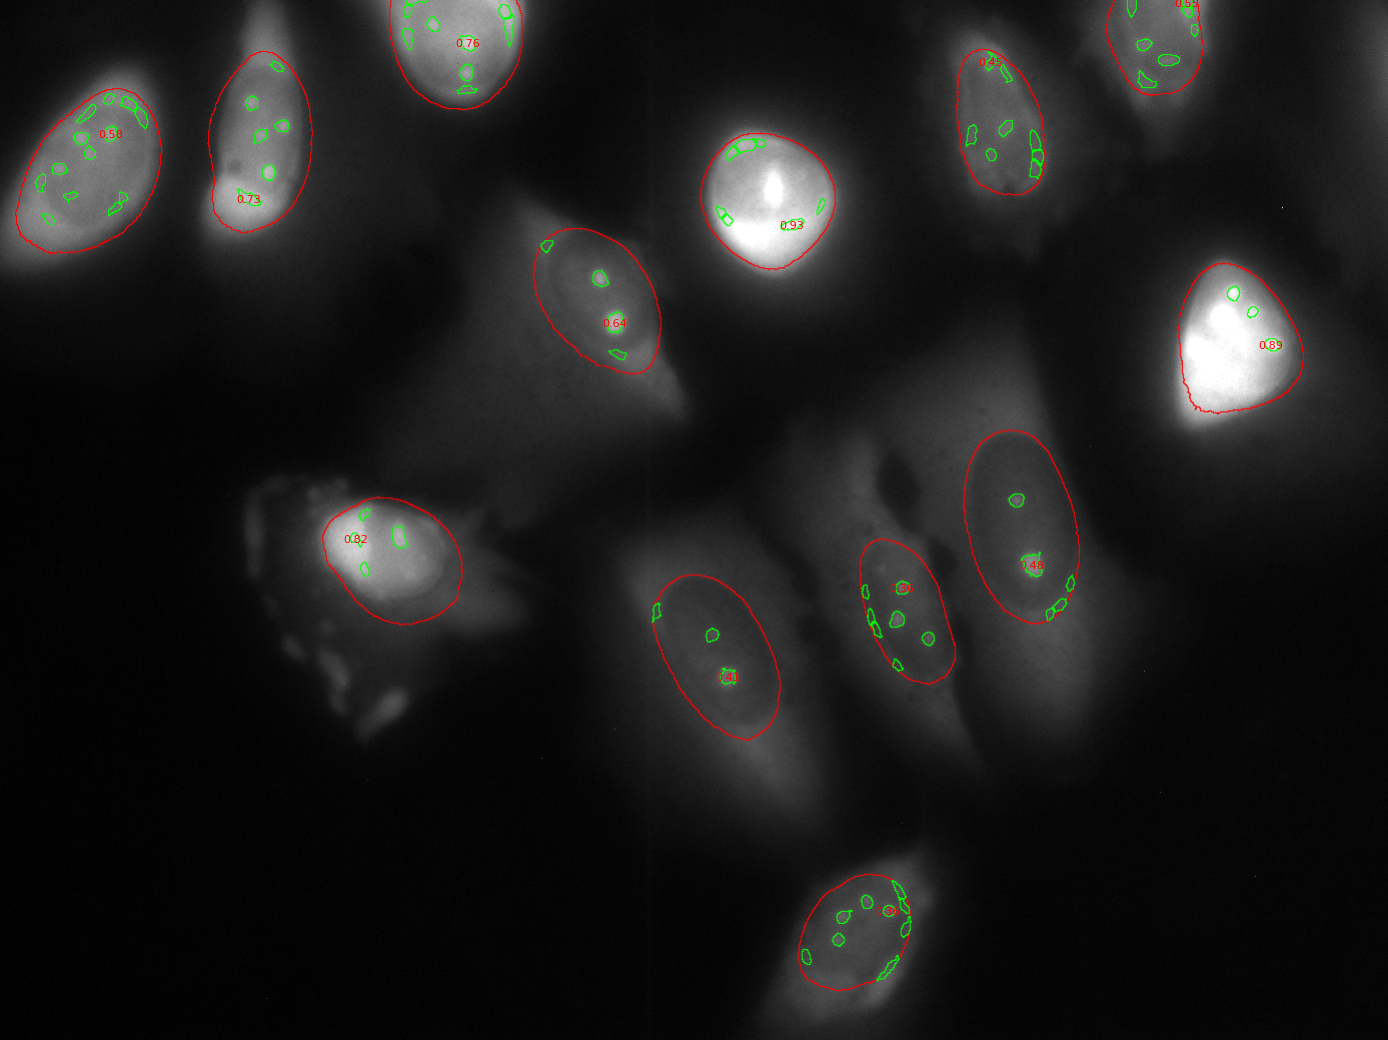
\includegraphics[width=\linewidth]{images/cellprofiler_channel1}
\caption{Example analysis performed with CellProfiler}
\label{fig:cellprofiler_example}
\end{figure}

\newpage
\section{Requirements}\label{sec:requirements}
The application has to meet the following requirements:
\begin{itemize}
  \item \textbf{Reliable nucleoli detection:} Stable and reliable detection of
  nucleoli is the main purpose of the application. Hence, it is supposed to
  detect at least 75\% of the nucleoli CellProfiler can detect. This includes
  a certain degree of stability concerning fuzzy pictures or pictures with
  unequally distributed or diffuse brightness.
  \item \textbf{Fast analysis:} As the application is tailored to this single
  task, it is expected to detect a suitable amount of nucleoli in only a small
  fraction of the time required by CellProfiler. The topmost time that the
  application may require to complete the analysis of one image is five seconds.
  \item \textbf{Fallback in case of empty nuclei:} Each nucleus is expected to
  containing at least one nucleolus. Yet, this expectation cannot always be
  fulfilled due to potentially damaged nuclei, fuzzy images, or other reasons.
  In this case, the center of the nucleus has to be provided as fallback target.
  \item \textbf{Visualizer:} In order to quickly check the results directly
  after running the analysis and to provide a way to quickly present the results
  to a potential audience, the application has to provide the possibility to be
  configured so that it shows the results as an image. This image has to contain
  all detected neuleoli targets, fallback targets and the regions of interest,
  e.g. the nuclei.
  \item \textbf{Versatility:} Since the appearance of different specimen can
  vary in various ways, all analysis parameters have to be configurable. Among
  others, this includes the minimum and maximum sizes of nuclei and nucleoli.
  The configuration is supposed to be achieved via an understandable,
  interchangeable, text-based file\footnote{Configurable parameters are
  explained in detail in the User's Manual section}.
  \item \textbf{Statistics:} To determine the most suitable parameters for
  different kinds of specimen, another feature may be configured. This
  statistics feature has to include:
  \begin{itemize}
    \item The amount of detected nuclei
    \item The amount of detected nucleoli
    \item Nuclei to nucleoli ratio as percentage
    \item The distance of each detected nucleolus to the center point of the
    containing nuclei and the average distance in pixels
    \item The area of each detected nucleus and the average area in square
    pixels
    \item The area of each detected nucleolus and the average area in square
    pixels
  \end{itemize}
  \item \textbf{Serialization of the results:} All results have to be stored in
  their accordant files in a subfolder \textit{results} of the folder
  containing the original data. The name of each result file has to contain a
  the timestamp indicating the application's execution in the format
  \newline \code{<year>\_<month>\_<day>\_<hour>\_<minute>\_<second>}.
  \newline E.g. \code{targets\_2014\_11\_20\_14\_50\_35.txt}.
  
  In the following, the accordant formats and files are described.
  \begin{itemize}
    \item \textbf{Targets:} Real targets and fallback targets sre to be saved in
    one txt-file named \code{targets\_<timestamp>.txt} in the
    following format:
    \begin{lstlisting}[caption=Format of results txt-file]
# nucleoli targets
<target number> : [<x-coord>, <y-coord>]
...
# targets in center of empty nuclei
<target number> : [<x-coord>, <y-coord>]
...
\end{lstlisting}

\textbf{Example:}
\begin{lstlisting}[caption=Example of results file]
# nucleoli targets
1 : [468, 43]
2 : [1183, 14]
# targets in center of empty nuclei
3 : [87, 174]
4 : [769, 198]
\end{lstlisting}
\item \textbf{Statistics:} The statistics as mentioned above have to be
stored in a txt-file named
\code{statistics\_<timestamp>.txt}. An example of the
statistics file can be found in the appendix.
\item \textbf{Result image:} The image as it would be displayed by the
visualizer has to be stored to a file named

\code{targets\_<timestamp>.<original image filetype>}. See Figure
\ref{fig:target_image_example} for an example the image.
\begin{figure}[h]
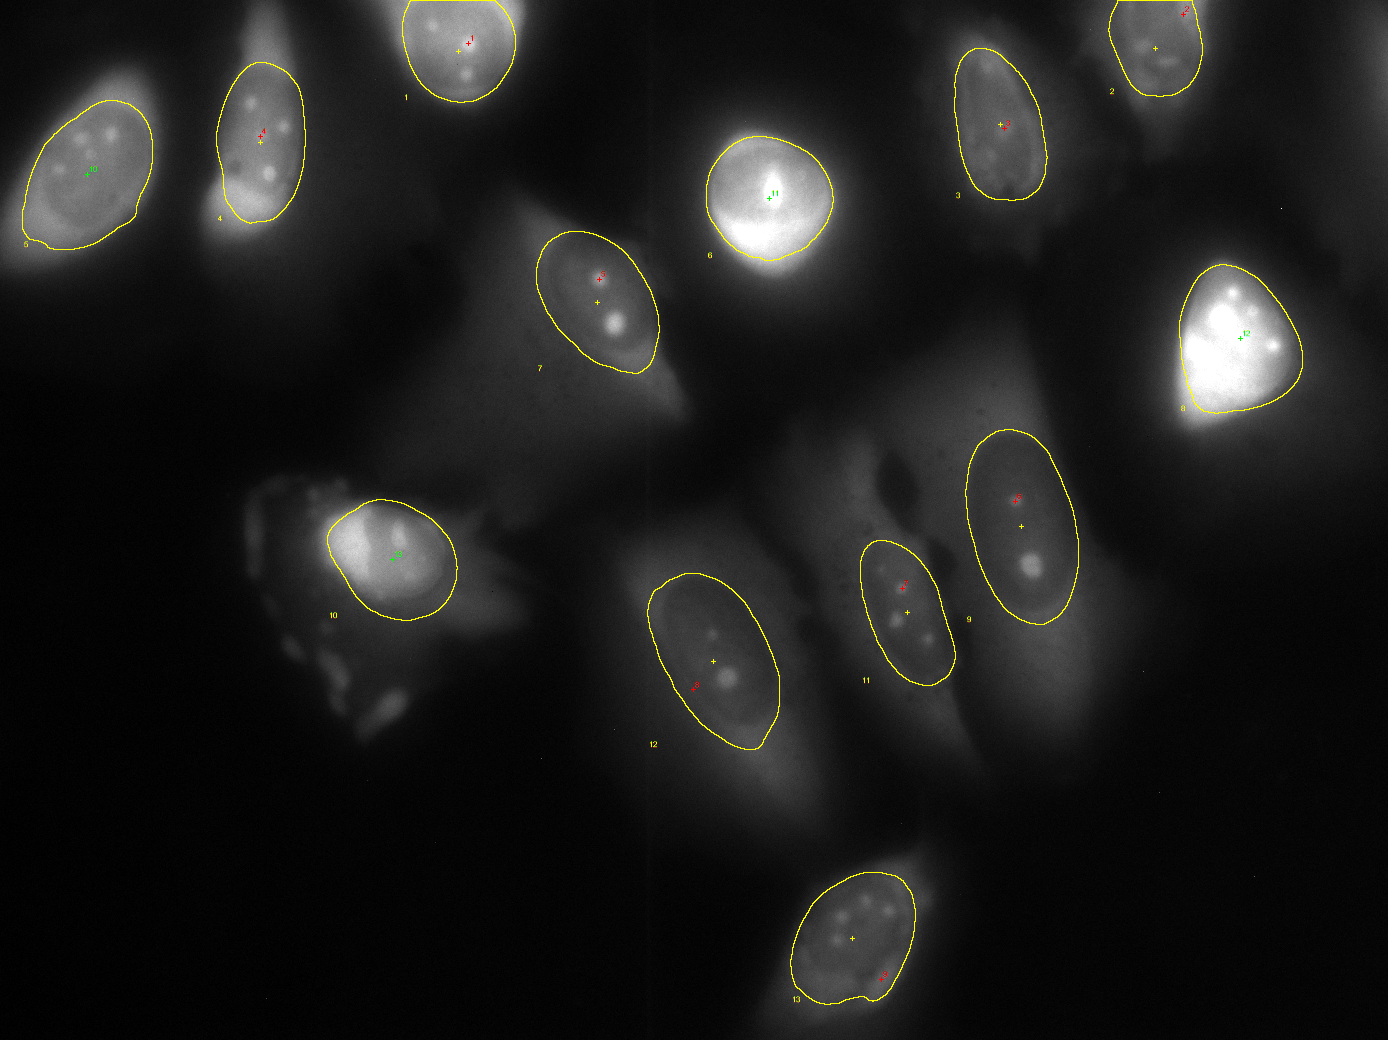
\includegraphics[width=\linewidth]{images/targets_example}
\caption{Example of the image containing the results}
\label{fig:target_image_example}
\end{figure}
  \end{itemize}
  \item \textbf{Quick and easy deployment:} The application is supposed to be
  deployed and run as easily as possible. Since the environment and the machines
  this will happen on may vary drastically, a versatile and independent way to
  do this is required. The Java framework delivers this possibility. Hence, the
  application will be developed using Java.
  \item \textbf{Use of an established graphics framework:} In
  order to keep maintenance effort as small as possible and, in case of
  potential future development, time it takes the developer to familiarize with
  the project, as short as possible, an established and well documented graphics
  framework has to be used. ImageJ meets these requirements and furthermore can
  be easily used as a library within a Java application.
\end{itemize}

\newpage
\section{User's Manual}

\subsection{System Requirements}
The application requires the Java Runtime Environment 1.7 or higher. For
Microsoft Windows 64bit operating system this results in the following minimum
system requirements \footnote{Further details on the system requirements can be
found at:
https://docs.oracle.com/javase/7/docs/webnotes/install/}:

\begin{table}[h]
\centering
\begin{tabular}{ l | r }
Memory: & 128MB \\
\hline
Processor: & Pentium 2 @ 266MHz \\
\hline
Disc space: & 124 MB + 2 MB \\
\end{tabular}
\caption{Minimum system requirements of Java 1.7 on Windows 64bit}
\label{tab:system_requirements_java7}
\end{table}

As it is good practice and vital to the security of any system, the Java
framework should be updated on a regular basis. Note that the requirements may
change with any update.

\subsection{Starting the Application}
Starting the application is accomplished using the command line interface via
Java's \code{java -jar} or \code{javaw -jar} command\footnote{See
https://docs.oracle.com/javase/7/docs/technotes/tools/windows/java.html for
further details.}. Furthermore, the application expects the configuration file
to be passed as single parameter.

Considering a scenario in which the configuration file (see \ref{sec:configuration}) is
stored as \code{configuration.txt} in the same folder as the \code{NuFi.jar}, the
following command will properly start the application:
\newline\code{java -jar NuFi.jar configuration.txt}.


\subsection{Configuration}\label{sec:configuration}
Configuration of the application is performed using a simple text file
containing the information listed in the following. Note that a missing
parameter will result in a fatal error, preventing the application from properly
working.

A complete example of the configuration file can be found in the appendix.

\subsubsection{General Parameters}
This section contains information on filetypes, source folders and naming
convention of source files.
\begin{itemize}
  \item \textbf{Source folder:} The folder containing the source files (e.g.
  image files) on which the analysis will be based. The source folders are
  expected to be provided as absolute path or relative to \code{NuFi.jar}.
  
  Note that the application expects exactly three files of the type defined as
  channel filetype. If there are more or less than three files of that type, a
  fatal error will occur.
  
  \textbf{Key:}
  \newline \code{source.folder}
  
  \textbf{Examples:}
  \newline \code{source.folder = C:/example/images}
  \newline \code{source.folder = ../../example/images}
  \newline \code{source.folder = example/images}
  
  \item \textbf{Used channels:} Each specimen is photographed three times
  using different colorization. This results in three different images
  referred to as different channels. Channels 1 and 3 are used in the process
  of detecting targets, thus, the correct specification and order of the
  files is vital for image analysis. Position one determines channel 1,
  position 3 determines channel 3. The source folder is scanned for files
  containing these channels determination. If these are not found, the
  application will terminate with a fatal error.
  
  \textbf{Key:}
  \newline \code{used.channels}
  
  \textbf{Examples:}
  \newline \code{used.channels = Kanal1, Kanal2, Kanal3}
  \newline \code{used.channels = channel1, channel2, channel3}
  
  \item \textbf{Channel filetype:} Though using the png-file format is advised,
  the application is built to be able to analyze various image formats. If it
  is necessary to analyze images that are not provided in the png-format, the
  accordant format can be provided using this key.
  
  \textbf{Key:}
  \newline \code{channel.filetype}
  
  \textbf{Examples:}
  \newline \code{channel.filetype = png}
  \newline \code{channel.filetype = jpg}
\end{itemize}
\subsection{General Picture Analysis Settings}
This section contains information of the expected size and shape of nuclei and
nucleoli, as well as the width of the in depth-analysis.

\begin{itemize}
  \item \textbf{Size settings:} Since the size of the nuclei and nucleoli in the
  specimen may vary and since the magnification of the microscope used in taking the
  pictures may also change, the size in the photographs may need to be adapted.
  This can be achieved by giving an average size in square-pixels and the
  minimum and maximum sizes as multiples of that size.
  
  \textbf{Keys:}
  \newline \code{nucleus.average}
  \newline \code{nucleus.min.factor}
  \newline \code{nucleus.max.factor}
  \newline \code{nucleolus.average}
  \newline \code{nucleolus.min.factor}
  \newline \code{nucleolus.max.factor}
  
  \textbf{Examples:}
  \newline \code{nucleus.average = 10000}
  \newline \code{nucleus.min.factor = 0.5}
  \newline \code{nucleus.max.factor = 1.5}
  \newline \code{nucleolus.average = 100}
  \newline \code{nucleolus.min.factor = 0.75}
  \newline \code{nucleolus.max.factor = 1.8}
  
  \item \textbf{Minimum circularity:} This parameter pays respect to the
  variation of the objects in their shape. A value of 1 indicates a perfect
  circle, while a 0 indicates that there are no requirements to the shape of the
  object. Since nuclei typically are elliptical in shape, a value of
  approximately 0.6 is advised. Nucleoli are typically close to a perfect
  circle.
  Thus, a value of 0.9 includes most of them while it excludes a variety of
  anomalies and prevents false-positives on nuclei borders.
  
  \textbf{Keys:}
  \newline \code{nucleus.min.circularity}
  \newline \code{nucleolus.min.circularity}
  
  \textbf{Examples:}
  \newline \code{nucleus.min.circularity = 0.6}
  \newline \code{nucleolus.min.circularity = 0.9}
  
  \item \textbf{In-depth width:} This parameter defines the variation in
  thresholding used during in-depth analysis.
  
  \textbf{Key:}
  \newline \code{indepth.range}
  
  \textbf{Examples:}
  \newline \code{indepth.range = 25}
  \newline \code{indepth.range = 10}
  
\end{itemize}

\subsubsection{Improved Image Detection Parameters}
In the standard setting the application will use the improved image detection
algorithm. In this section, the parameters required for this algorithm can be
defined. These include setting for brightness correction
(\code{<object>.background.blur} and \code{<object>.thresholding.blur}) and the
value used for correcting discrepancies between channel 3 colorization and the
actual size of nuclei (\code{nucleus.boundary.width}).

\begin{itemize}
  \item \textbf{Brightness correction:}
\end{itemize}

\textbf{Keys:}
\newline \code{nucleus.background.blur}
\newline \code{nucleus.thresholding.blur}
\newline \code{nucleus.boundary.width}
\newline \code{nucleolus.background.blur}
\newline \code{nucleolus.thresholding.blur}

\textbf{Examples:}
\newline \code{nucleus.background.blur = 100}
\newline \code{nucleus.thresholding.blur = 3}
\newline \code{nucleus.boundary.width = 5}
\newline \code{nucleolus.background.blur = 10}
\newline \code{nucleolus.thresholding.blur = 1}


\subsection{Structure of Files and Folders}
\begin{figure}
\centering
\raisebox{-\height}{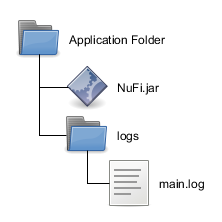
\includegraphics[width=120px]{images/folders_application}}
\raisebox{-\height}{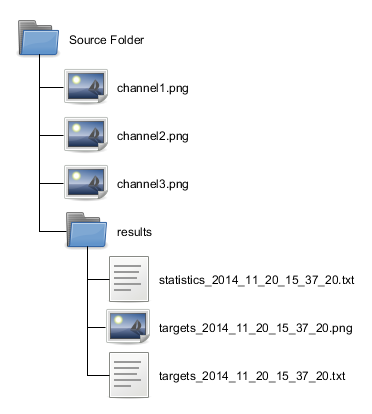
\includegraphics[width=200px]{images/folders_data}}
\caption{Structure of directories and files created in the application's
folder and the source folder}
\label{fig:folders}
\end{figure}

The results of the image analysis will be stored into a directory \code{results}
which is created as a subfolder of the directory defined as source folder. This
directory will contain the targets file, the result image and, in case
statistics are enabled, the statistics file. See figure \ref{fig:folders}.

The application will neither delete nor overwrite files created by a previous
execution since each file contains a timestamp as defined in
\ref{sec:requirements}.

Besides this, the application will create a directory \code{logs} on the same
level as \code{NuFi.bat} is located. This directory contains the log-file of the
application itself. If any unexpected behaviour is encountered while using the
application, refer to this file since it might contain helpful information. See
figure \ref{fig:folders}.

\newpage
\section{Image Analysis}

In this section the procedure of how the application processes and analyzes
images is explained. Details such as how the applications checks its
configuration are omitted in favor of more emphasis on image analysis.

\begin{figure}[h]
\centering
\begin{subfigure}[b]{0.48\textwidth}
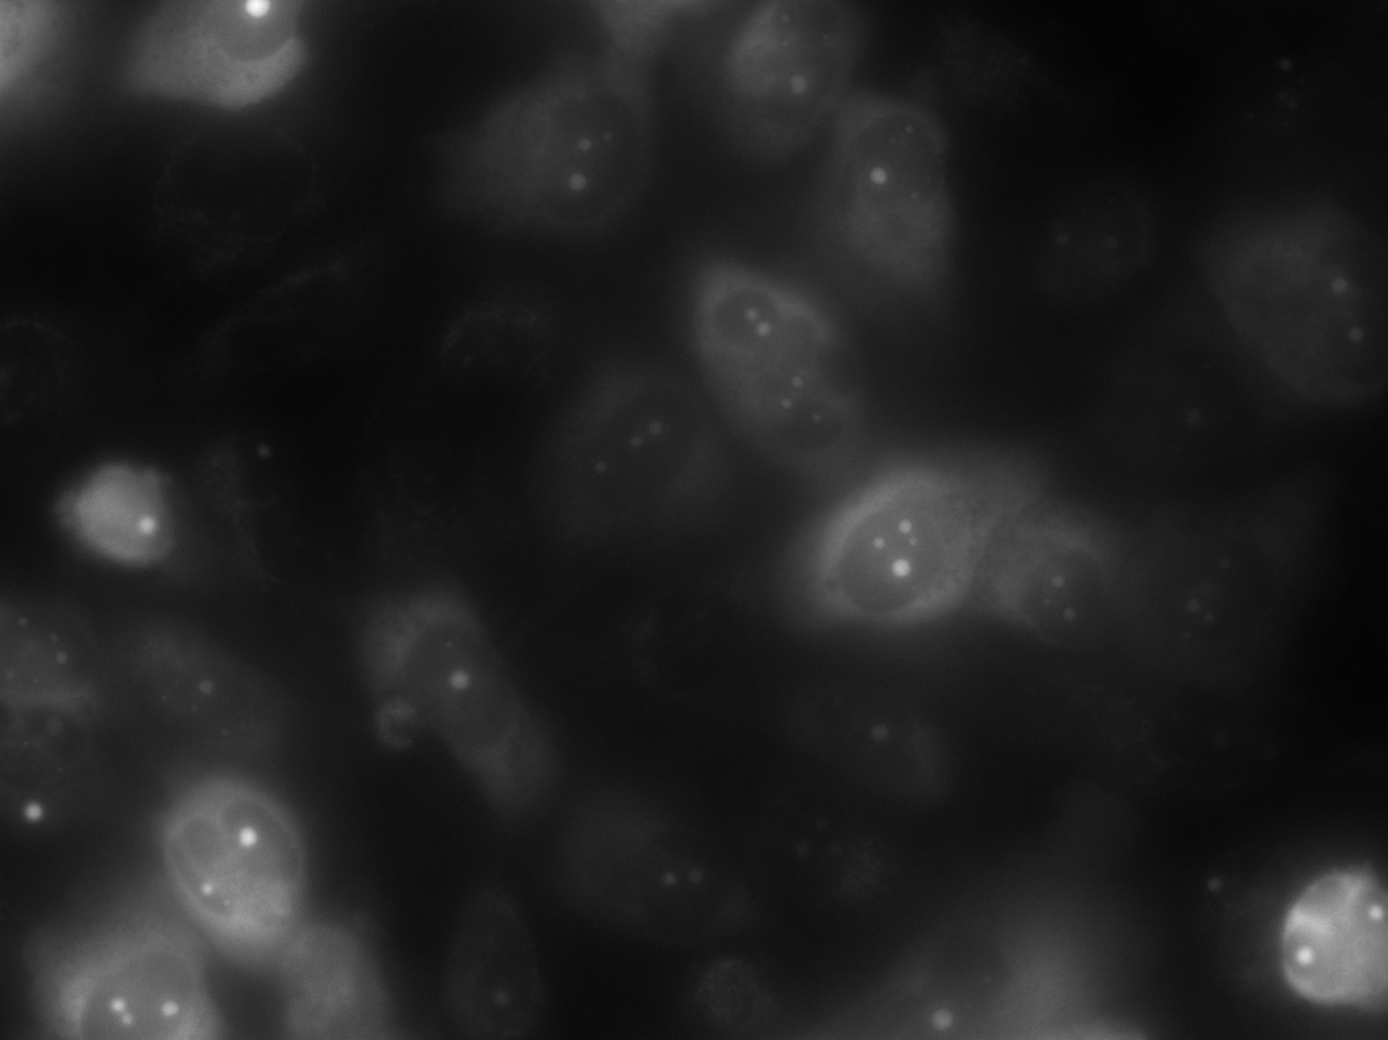
\includegraphics[width=\textwidth]{images/example_Kanal1}
\caption{Channel 1 example image}
\end{subfigure}
\begin{subfigure}[b]{0.48\textwidth}
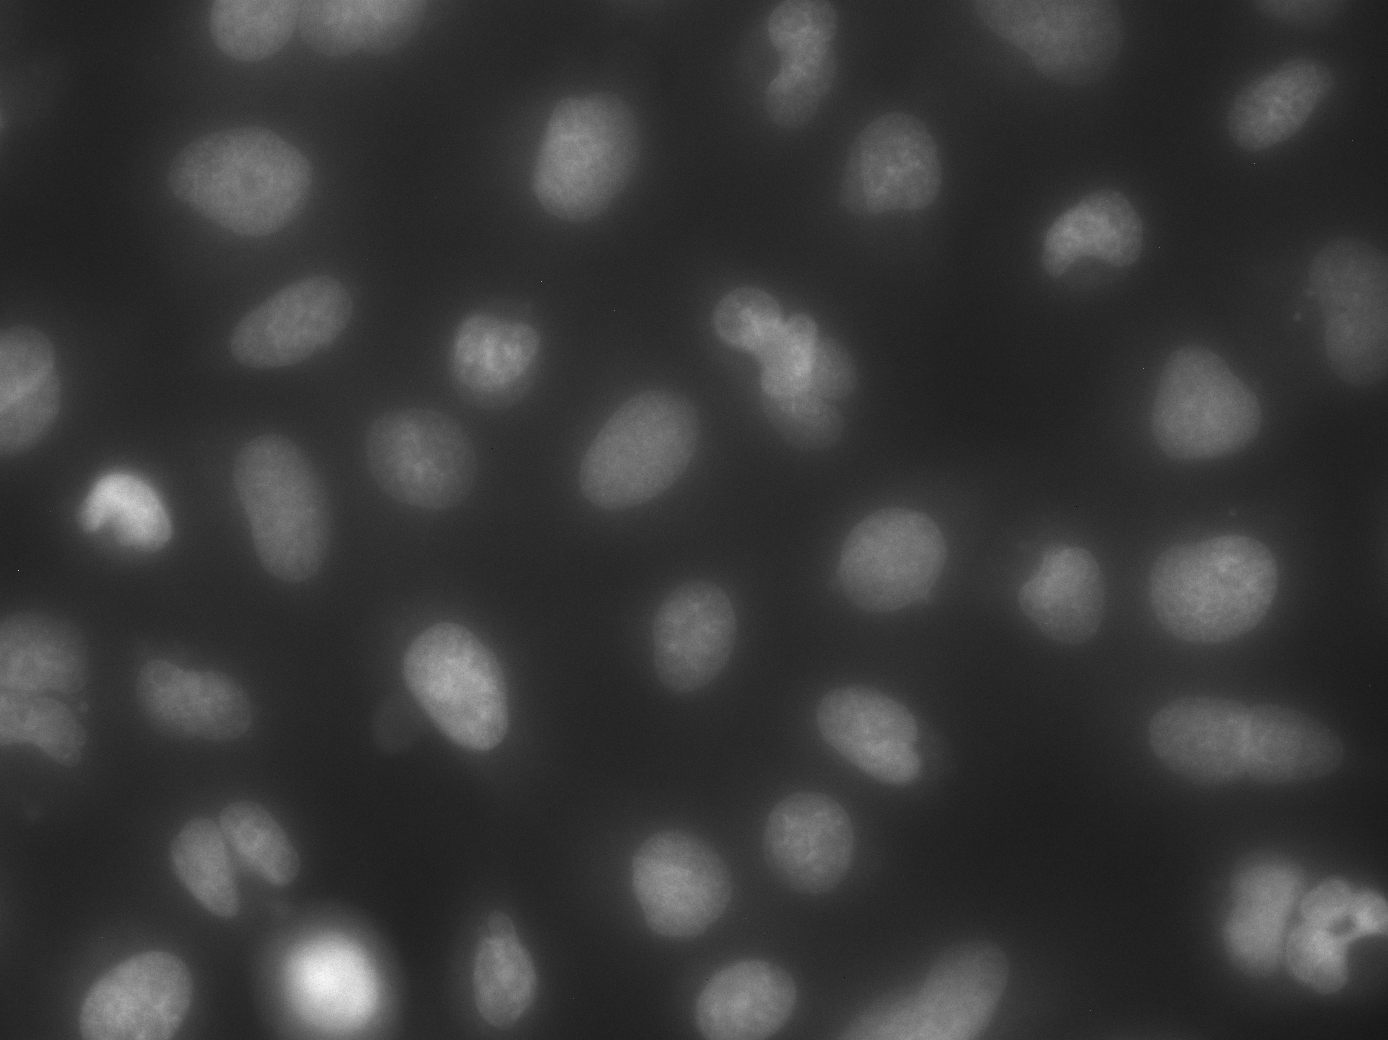
\includegraphics[width=\textwidth]{images/example_Kanal3}
\caption{Channel 3 example image}
\label{fig:channel3}
\end{subfigure}
\caption{Example images of channel 1 and 3}
\label{fig:example_images}
\end{figure}

\subsection{Target Detection Procedure}
The target detection process can basically divided in two parts. At first, the
regions of interest are detected using channel 3. These regions are then
transferred to channel 1 in order to only analyze those regions that may
actually contain nucleoli.

In the following, these two parts are explained step-by-step using the example
images in figure \ref{fig:example_images}.


\subsubsection{Determining Regions of Interest}

\begin{wrapfigure}{r}{0.33\textwidth}
\vspace{-14pt}

\includegraphics[width=0.3\textwidth]{images/example_Kanal3_gaussian100}
\caption{Channel 3 after Gaussian Blur with a radius of 100 pixels has been
applied}
\label{fig:example_channel3_gaussian}
\vspace{-28pt}
\end{wrapfigure}
Finding the regions of interest is performed using only the image referred to as
channel 3, as this is the image which best shows the nuclei due to the
colorization used.

Typically the images show very uneven exposure to light, resulting in the
necessity of brightness correction as a very first step. This is achieved by
using a gaussian blur with a radius approximately the size of the objects that
are supposed to be found, in this example, a value between 100 and 120 yields
pretty useful results. The result of this operation can be seen in
\ref{fig:example_channel3_gaussian} and is referred to as background image. The
original channel 3 image is then divided by the background image, which means
that each pixel value of the original image is divided by the value of the pixel
of the background image that is at the same location. 
This leads to an image with very small pixel values, typically close to zero,
e.g. the resulting image is all black. Consequently, the next step is to
multiply each pixel value with a constant factor, e.g. 178. As a last step in
this preparation process, a gaussian blur with a small radius, e.g. 2px, is
applied to the image in order to smooth the edges of the nuclei and to reduce
noise. The result of these steps can be seen in \ref{fig:example_channel3_prepared}.

\begin{wrapfigure}{l}{0.33\textwidth}
\vspace{-14pt}
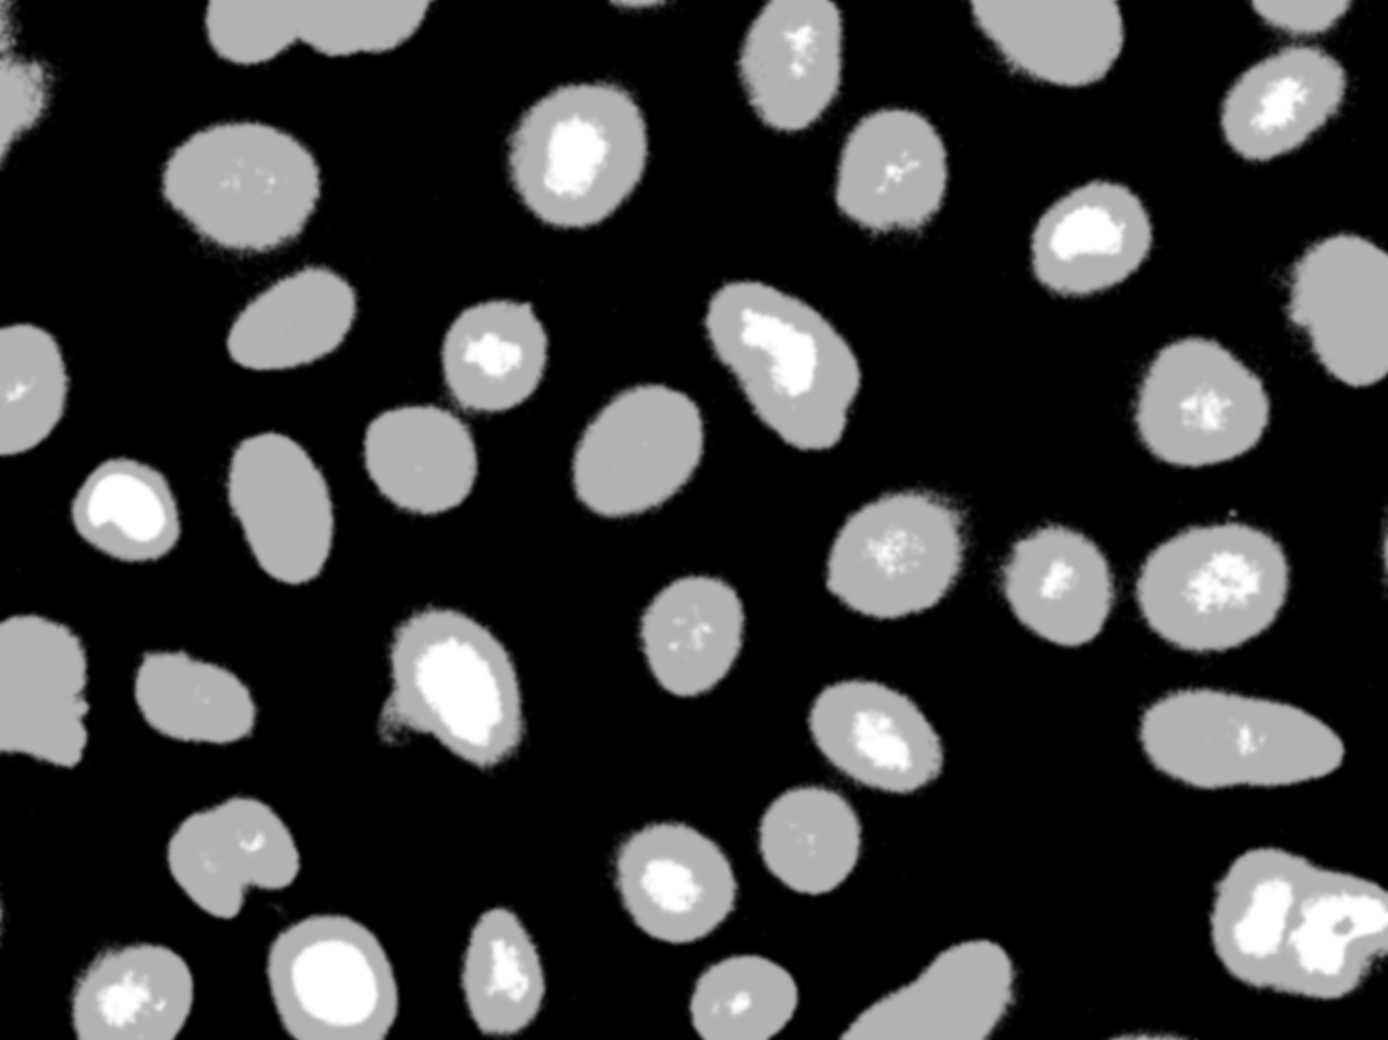
\includegraphics[width=0.3\textwidth]{images/example_Kanal3_multiply178_gaussian2}
\caption{Channel 3 after brightness correction has been performed}
\label{fig:example_channel3_prepared}
\end{wrapfigure}

Having finished this preparation, channel 3 now shows evenly distributed
brightness and only little variation in these. This makes the following step,
finding a suitable threshold which is described in detail in
\ref{sec:thresholding}, easier and much more stable across different images.
Figure \ref{fig:channel3_threshold} shows channel 3 after an auto
default threshold was applied.

\begin{wrapfigure}{r}{0.33\textwidth}
\vspace{-14pt}
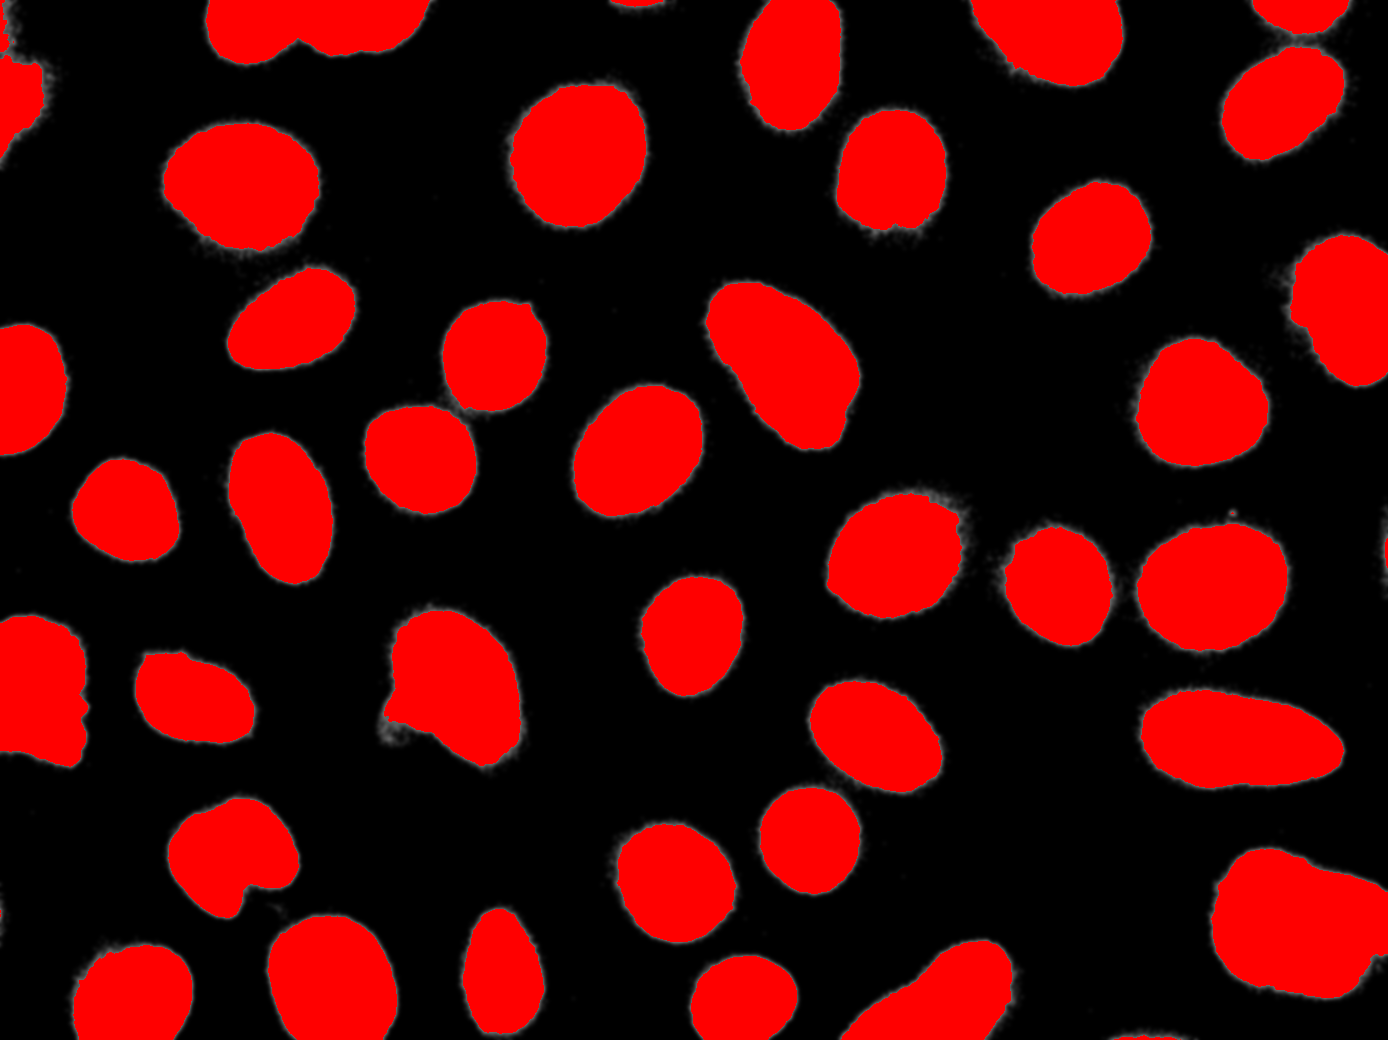
\includegraphics[width=0.3\textwidth]{images/example_Kanal3_corrected_threshold}
\caption{Channel 3 with auto threshold applied}
\label{fig:channel3_threshold}
\end{wrapfigure}

In the last part of determining the regions of interest, the areas to which the
threshold applies, e.g. are marked in red, are analyzed using ImageJ's
Particle Analyzer plugin. Details on how Particle Analyzer works are explained
in \ref{sec:particle_analysis}. Based on configured values for minimum and
maximum area a nucleus may cover and minimum circularity, the regions of
interest are determined. Figure \ref{fig:channel3_rois} shows the result of
running a particle analysis on figure \ref{fig:channel3_threshold} using a
minimum area of 8000 pixel$^2$, a maximum area of 15000 pixel$^2$ and a minimum
circularity of 0.6. Obviously, not all nuclei are recognized as reagions of
interest. In this example, the area of these nuclei are too large or too small.
If the specimen contains a vast amount of too large or too small nuclei,
changing the configured minimum and maximum sizes should be adapted. 

The regions of interest determined in this first part of the image analysis are
the basis of finding nucleoli in the next step. If these regions cannot be
properly determined, for example due to low quality images or flawed
colorization, the subsequent analysis will not yield feasible results.

See appendix for high resolution versions of the images used in this section.

\begin{figure}[h]
\centering
\fbox{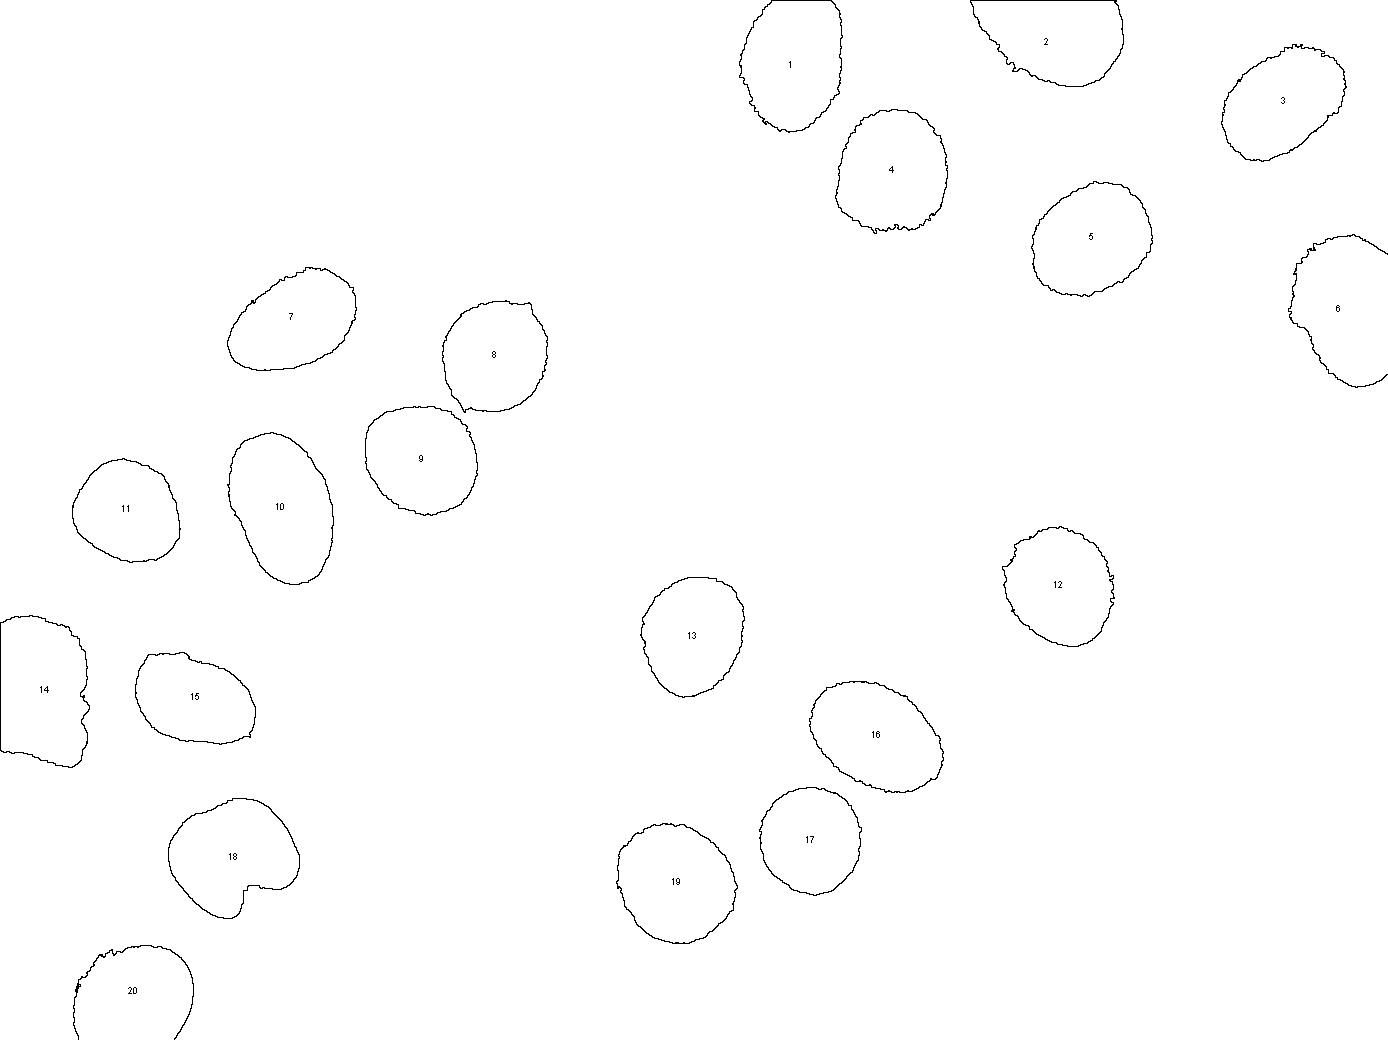
\includegraphics[width=0.8\textwidth]{images/example_Kanal3_rois}}
\caption{Regions of interest found by Particle Analyzer in thresholded channel 3
image}
\label{fig:channel3_rois}
\end{figure}

\subsubsection{Finding Nucleoli}

\begin{wrapfigure}{l}{0.33\textwidth}
\vspace{-14pt}
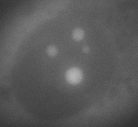
\includegraphics[width=0.3\textwidth]{images/example_nucleus}
\caption{Example nucleus}
\label{fig:example_nucleus}
\vspace{-28pt}
\end{wrapfigure}
Having found the regions of interest, the area which has to be searched is
drastically reduced. Furthermore, since each region is analyzed separately,
influence from uneven exposure to light is negligible. Hence, in favor of
faster execution no further brightness correction is performed while detecting
nucleoli. The following describes the process by the example of one region of
interest, e.g. one nucleus. Nonetheless, in the whole process of target
detection, this process is performed for each region of interest. The example
nucleus can be seen in figure \ref{fig:example_nucleus}.

The first step in order to analyze a single nucleus is to crop the affected
region as seen in \ref{fig:example_nucleus}. Apparently, the region of interests
border does not exactly match the boundaries of the nucleus. This is caused by
the differences in colorization of channel 1 and 3 and by a delay between taking
the pictures. Furthermore, the colorization of channel 1 causes the boundaries
of nuclei to be nearly as bright as the nucleoli. Without proper correction
false-positives are likely to appear on the boundaries. To counter this, the
extend of the region of interest is shrunk by the configured amount of pixels.
Additionally, in order to prevent the brightness outside the region of interest,
all pixels that are not inside the region, are set to black. This results in the
image depicted in figure \ref{fig:example_nucleus_shrinked_blacked}.

\begin{wrapfigure}{r}{0.33\textwidth}
\vspace{-14pt}
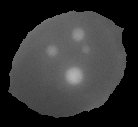
\includegraphics[width=0.3\textwidth]{images/example_nucleus_shrinked8_blacked}
\caption{Region of interest shrunk by 8 pixels, everything outside the region
is set to black}
\label{fig:example_nucleus_shrinked_blacked}
\end{wrapfigure}

After preparing the image of the nucleus like this, the analysis is continued by
applying an auto determined threshold using ImageJ's auto thresholding
procedures. In contrast to determining the regions of interest, where all
thresholding methods lead to comparable results, different methods lead to
significantly different results when applied here. Figure
\ref{fig:threshold_comparisson} shows the effects of different thresholding
methods.

By comparing the results of different thresholding methods applied to numerous
nuclei found in several pictures, the MaxEntropy method, depicted in figure
\ref{fig:threshold_maxentropy}, was determined as the most suitable one.

\begin{figure}[h]
\centering
\begin{subfigure}[b]{0.23\textwidth}
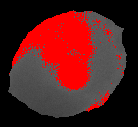
\includegraphics[width=\linewidth]{images/example_nucleus_threshold_default}
\caption{Default}
\end{subfigure}
\begin{subfigure}[b]{0.23\textwidth}

\includegraphics[width=\linewidth]{images/example_nucleus_threshold_huang}
\caption{Huang}
\end{subfigure}
\begin{subfigure}[b]{0.23\textwidth}
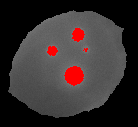
\includegraphics[width=\linewidth]{images/example_nucleus_threshold_maxentropy}
\caption{MaxEntropy}
\label{fig:threshold_maxentropy}
\end{subfigure}
\begin{subfigure}[b]{0.23\textwidth}
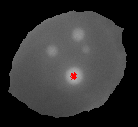
\includegraphics[width=\linewidth]{images/example_nucleus_threshold_shanbhag}
\caption{Shanbhang}
\end{subfigure}
\caption{Comparisson of different thresholding methods}
\label{fig:threshold_comparisson}
\end{figure}

Based on the threshold achieved by using the MaxEntropy method, a particle
analysis is performed similar to the one performed to determine the regions of
interest, but with parameters that pay respect to the size and shape of nucleoli
rather than nuclei. Figure \ref{fig:example_nucleus_shrinked_blacked} shows the
result of an analysis with a minimum size of 80 pixel$^2$, a maximum size of 350
pixel$^2$ and a minimum circularity of 0.8. Note that the nucleolus on the
right is not recognized due to the fact that it is smaller than the configured
minimum size.

\begin{figure}[h]
\centering
\begin{subfigure}[b]{0.25\textwidth}
\fboxsep=0.5mm
\fbox{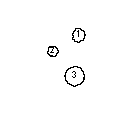
\includegraphics[width=\textwidth]{images/example_nucleus_rois}}
\caption{Plain regions of interest}
\end{subfigure}
\quad
\begin{subfigure}[b]{0.25\textwidth}
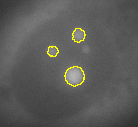
\includegraphics[width=\textwidth]{images/example_nucleus_rois_overlay}
\caption{Regions of interest as overlay}
\end{subfigure}
\caption{Regions of interest found by particle analysis}
\end{figure}

To determine which of the nucleoli found is the most suitable target, the sizes
of all nucleoli within one nucleus are compared. In order to ensure high
accuracy during exposure to radiation later on in the process of analyzing the
specimen, the largest nucleolus, e.g. covers the largest area, is chosen. Note
that this will not result in choosing too large objects, since these are ignored
due to the maximum size defined in particle analysis. In the example nucleus,
region 3 is determined the most suitable choice, which can bee seen in figure
\ref{fig:example_nucleus_target}. 

\begin{figure}
\centering
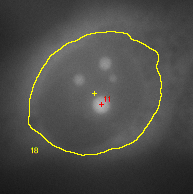
\includegraphics[width=0.3\textwidth]{images/example_nucleus_target}
\caption{Extract from the result image showing the example nucleus as well as
the chosen target}
\label{fig:example_nucleus_target}
\end{figure}

In case no nucleoli are found in a certain nucleus, the application acts on the
assumption that all nuclei contain at least one nucleolus and thus performs an
in-depth analysis of the nucleus. This analysis is performed by using different
thresholds based on the automatically found threshold and the configured width
of the in-depth analysis. The nucleus will be thresholded with values of
\code{threshold - inDepthWidth} to \code{threshold - inDepthWidth}. By
stepwise increasing the threshold's value the possibility of not finding a
nucleolus due to the fact hat it is just outside the minimum or maximum size
because of a sub-optimal threshold is reduced. As soon as one nucleolus is
found, the in-depth analysis is finished.

\subsection{Thresholding}\label{sec:thresholding}
Despite the possibility of determining the threshold by hand or, respectively
newly implement ways of automatically finding a suitable threshold, the
application relies on ImageJ's AutoThresholder. This ImageJ plugin provides the
possibility to use different algorithms(also: methods) to determine the
threshold automatically.
These include algorithms such as Huang \cite{huang93}, Otsu \cite{green10},
MaxEntropy \cite{fiji04} and others\footnote{\cite{landini13} provides an
elaborated overview on the AutoThresholder plugin and the available methods.}.

This section is intended to give a brief overview of how thresholding in general
and the two methods used here, default and MaxEntropy, in particular, work. For
a more detailed explanation please refer to the cited sources as this is not
within the scope of this work.

Thresholding is used to simplify image analysis by reducing the information
contained within the image data. Typically this results in a binary, e.g. black
and white, image. This may be achieved by simply comparing a pixel's
(brightness) value to a defined value, the threshold. If the pixel's value is
below that threshold, the value is set to 0 (black), if it is above, the value
is set to 1 (white). Note that in some cases black and white may be switched in
order to ease further processing. A very basic approach to do this can be seen
in the below Java source code:

\begin{lstlisting}[language=Java, caption=Basic thresholding algorithm]
/*
width, height refer to the image's width and height

threshold refers to the predefined threshold

image.value(int x, int y) returns the value of the pixel at 
	position (x, y)

image.setValue(int x, int y, double newValue) sets the value 
	of the pixel at position (x, y) to newValue
*/

for (int x = 0; x < width; x++) {
	for (int y = 0; y < height; y++) {
		if (threshold > image.value(x, y)) {
			image.setValue(x, y, 0d);
		} else {
			image.setValue(x, y, 1d);
		}
	}
}
\end{lstlisting}

While this is pretty much the idea behind thresholding, there are several
sophisticated approaches on how to determine a suitable value to be used as
threshold based on an image's histogram and assumptions on how pixels are
related to each other. Figure \ref{fig:example_histograms} shows the histograms
of the original channel 3 image as shown in \ref{fig:channel3} and the
brightness corrected version as shown in figure
\ref{fig:example_channel3_prepared}. Apparently, finding a suitable threshold
based on the histogram is much easier in the brightness corrected version of
the image.

\begin{figure}[h]
\centering
\begin{subfigure}[b]{0.4\textwidth}
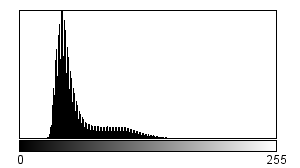
\includegraphics[width=\textwidth]{images/histogram_original}
\caption{Original image}
\end{subfigure}
\quad
\begin{subfigure}[b]{0.4\textwidth}
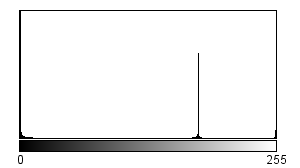
\includegraphics[width=\textwidth]{images/histogram_brightness_corrected}
\caption{After brightness correction}
\end{subfigure}
\caption{Histograms of channel 3 prior to brightness correction and afterwards}
\label{fig:example_histograms}
\end{figure}

The thresholding algorithm that is used in ImageJ by the name of
\textit{default} is basically a slight variation of the IsoData algorithm,
compare \cite{landini13}, which is also known as \textit{iterative intermeans} described
in \cite{ridler78}. This iterative algorithm defines an initial threshold as a
basis for the first iteration, typically half the dynamic range, e.g. 178 if
the range is 0 to 255. The algorithm then determines the average value of the
pixels below and above the threshold. The threshold for the next iteration is
then calculated as the  arithmetic mean of these two values. The algorithm
terminates when the value does not change anymore. The below source code shows
a possible implementation of this algorithm:



The second method used in the application is based on the entropy found in the
histogram \cite{kapur84}. According to \cite{fiji04} the MaxEntropy threshold of
a normalized histogram can be calculated as follows:
\begin{align*}
\sum_{i=0}^{i_{max}} h(i) = 1
\end{align*}
Indicating that the histogram $h$ is normalized, e.g. the sum of all
values $h(i)$ equals $1$. The entropy  $H_B$ of black pixels is defined as:
\begin{align*}
H_B(t) = - \sum_{i=0}^{t} \Bigg(\frac{h(i)}{ \sum_{j=0}^{t} h(j)}
log \frac{h(i)}{ \sum_{j=0}^{t} h(j)}\Bigg)
\end{align*}
while the entropy $H_W$ of white pixels is defined as:
\begin{align*}
H_W(t) = - \sum_{i=t+1}^{i_{max}} \Bigg(\frac{h(i)}{ \sum_{j=t+1}^{i_{max}}
h(j)} log
\frac{h(i)}{ \sum_{j=t+1}^{i_{max}} h(j)}\Bigg)
\end{align*}
The optimal threshold $T_{opt}$ is defined as the maximum of the sum of these
entropies:
\begin{align*}
T_{opt}=Max(H_B(t)+H_W(t)) \quad , \quad t \, \epsilon \, [0, i_{max}]
\end{align*}

In order to determine the optimal threshold, the basic form of this algorithm
calculates the entropies of black and white pixels for each possible threshold, e.g. 256
different values for $t$. This might seem extensive and time-consuming. Yet,
compared to other operations to be performed while analyzing the image, this is
put into perspective. Furthermore, the results this algorithms yields when
applied to images of single nuclei beat that of other algorithms considering
stability and effectiveness. Additionally, the possible values of $t$ can be
reduced by an analysis of the histogram prior to calculating the analysis.

\subsection{Particle Analysis}\label{sec:particle_analysis}

The ImageJ documentation on this topic is rather superficial. Nonetheless, the
basics of particle detection is some kind of Hough transformation as described
in \cite{duda71}. Since this is a rather elaborated technique with various
existing enhancements and modifications, this section will only describe the
basic technique by the example of detecting straight lines.

Nonetheless, ImageJ's documentation does state that ParticleAnalyzer works with
the following algorithm:

\begin{center}
\noindent\fcolorbox{black}{codegray}{%
\begin{minipage}{\dimexpr\linewidth-2\fboxsep-2\fboxrule\relax}
\begin{algorithmic}
\For {each line}
	\For{each pixel in this line}
		\If{pixel value ``inside'' threshold range}
		
			\State trace the edge to mark the object
			
			\State do measurements
		
			\State fill the object with a color outside threshold range
		\Else
		
			\State continue scan
		\EndIf
	\EndFor
\EndFor
\end{algorithmic}
\end{minipage}% 
}
\end{center}

Where \textit{``trace the edge to mark the object''} may refer to various
tracing algorithms, for example a Hough transformation. The basic idea behind
Hough transformations is to find a space in which the same information can be
represented in a more useful way. For example, if a simple straight line has to
be detected, the coordinates of the Hough space are not x and y coordinates, but
instead the angle between the line and the x-Axis and its distance to the
center of coordinates. By doing so, a line in carthesian space can be
represented by a single point in Hough space, as seen in figure 
\ref{fig:cathesian_hough}.

\begin{figure}[h]
\centering
\begin{subfigure}[b]{0.4\textwidth}
\fboxsep=0.5mm
\fbox{
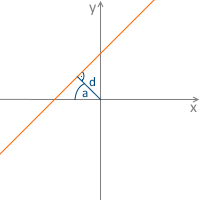
\includegraphics[width=\textwidth]{images/example_carthesian}
}
\caption{Straight line in carthesian coordinates}
\end{subfigure}
\quad
\begin{subfigure}[b]{0.4\textwidth}
\fboxsep=0.5mm
\fbox{
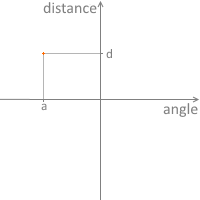
\includegraphics[width=\textwidth]{images/example_hough}
}
\caption{Single point in Hough space representing the same line}
\end{subfigure}
\caption{The same line represented in carthesian coordinates and in Hough space}
\label{fig:cathesian_hough}
\end{figure}

While this is a neat way of representing a straight line with known angle and
distance to the x-axis, finding a straight line within the data of an image
requires some more effort. The basic idea behind edge tracing with hough
transformations is to look at each pixel in the image\footnote{Note that the
image was thresholded beforehand thus is binary, e.g. only includes black and
white pixel, by the time the transformation is applied} and, given the pixel has
the desired foreground value, e.g. white, determines the distance $d$ between
the coordinate center a straight line for every possible angle $\alpha$ that
line's normal can enclose with the x-axis by calculating $d(\alpha) = x \cdot
\cos(\alpha) + y \cdot \sin(\alpha)$ for $\alpha \, \epsilon \, [0, \pi]$. The
graphs of $d(\alpha)$ for each point are then accumulated. This can be achieved
by the following algorithm:

\begin{center}
\noindent\fcolorbox{black}{codegray}{%
\begin{minipage}{\dimexpr\linewidth-2\fboxsep-2\fboxrule\relax}
\begin{algorithmic}
	\State $maxDistance \gets \sqrt{(\frac{1}{2} \cdot imageHeight)^2 +
	(\frac{1}{2} \cdot imageWidth)^2}$
	\State $minDistace \gets -maxDistance$
	\State $houghSpace[0..\pi][minDistance..maxDistance] \gets 0$
	\For{each line}
		\For{each pixel in that line}
			\If{$pixelValue = 0$}
				skip that pixel
			\EndIf
			\For{$\alpha \gets 0$ to $\pi$}
				\State $distance \gets x_{pixel} \cdot \cos(\alpha) + y_{pixel} \cdot
				\sin(\alpha)$ 
				
				\State $houghSpace[\alpha][distance]++$ 
			\EndFor
		\EndFor
	\EndFor
\end{algorithmic}
\end{minipage}% 
}
\end{center}

To determine the detected line's distance and angle, that point in Hough space
which has the overall maximum value has to be found, which can be simply done by
iterating over the values and comparing them. From that values angle $\alpha$
and distance $d$ the straight line can be reconstructed in the original
carthesian coordinate system. This is illustrated in figure
\ref{fig:example_lines_hough}\footnote{Image taken from
http://upload.wikimedia.org/wikipedia/commons/1/1c/Hough-example-result-en.png}.

\begin{figure}[H]
\centering
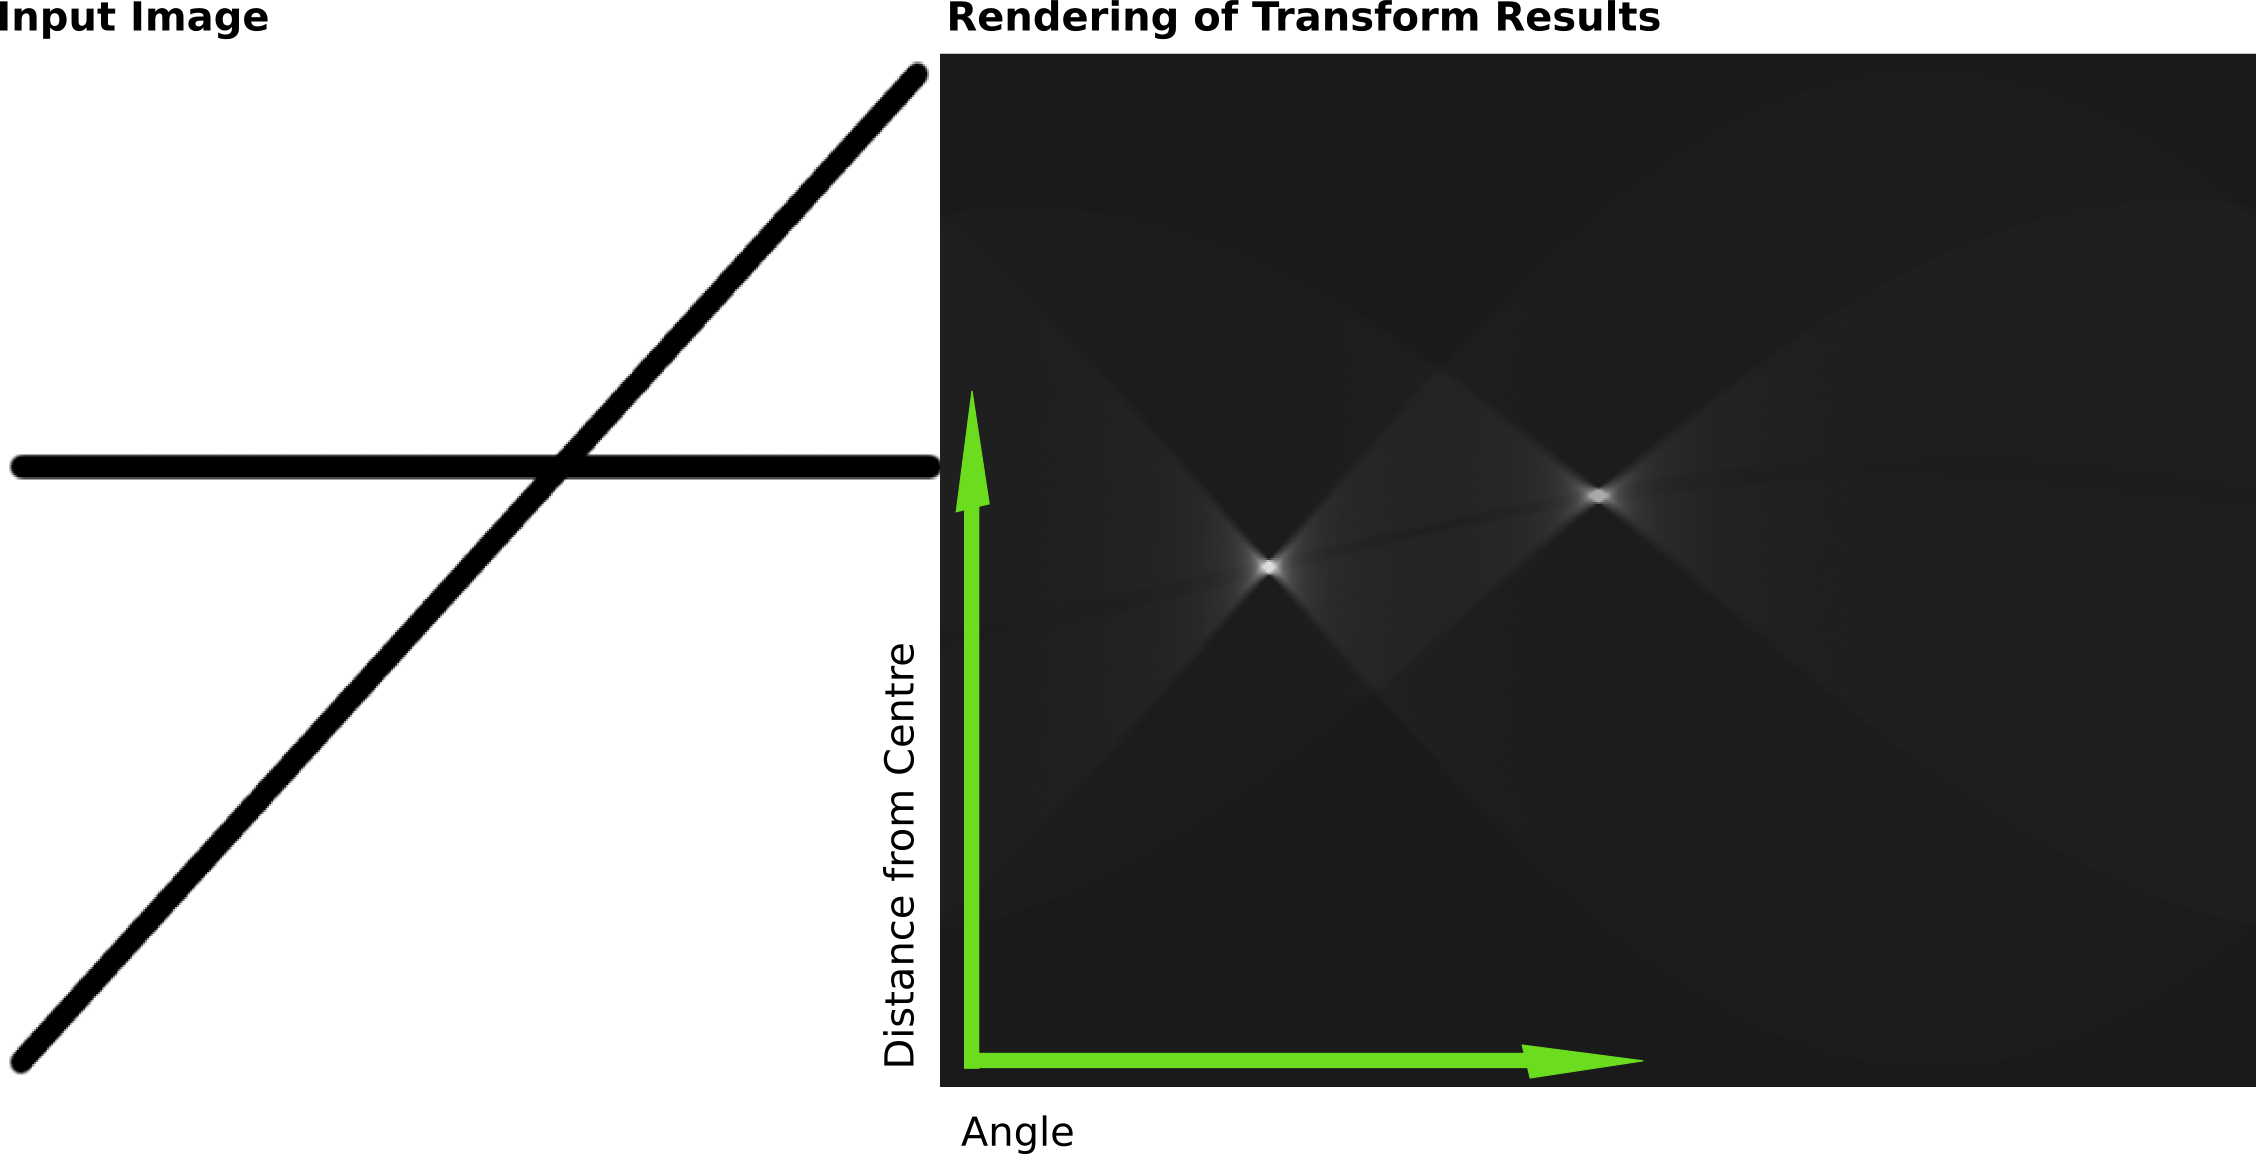
\includegraphics[width=\linewidth]{images/Hough-example-result-en}
\caption{Example of detecting lines using Hough
transformation}
\label{fig:example_lines_hough}
\end{figure}

In order to detect circles or arbitrary shapes, other parameters have to be
found. In the case of (overlapping) circles that are to be detected, Hough space
would be three dimensional, consisting of the center coordinates and radii of
the circles. Besides that and corresponding changes, the procedure stays the
same.

\newpage
\section{Conclusion and Prospect}

\subsection{Evaluation}
\label{sec:evaluation}
Evaluation happened on basis of 15 different sets of images taken in May 2014
which were analyzed using the following settings:

\begin{lstlisting}[caption=Settings used during evaluation]
nucleus.average = 10000
nucleus.min.factor = 0.4
nucleus.max.factor = 2.6
nucleus.min.circularity = 0.6

nucleolus.average = 100
nucleolus.min.factor = 0.5
nucleolus.max.factor = 4
nucleolus.min.circularity = 0.8

indepth.range = 30

# settings for improved mode
nucleus.background.blur = 100
nucleus.thresholding.blur = 3
nucleus.boundary.width = 5

nucleolus.background.blur = 10
nucleolus.thresholding.blur = 1
\end{lstlisting}

This lead to the results shown in \ref{tab:evaluation}. With the success rate
calculated as $\frac{(\#found - \#wrong)}{(\#found - \#wrong + \#missing)}$.
Note that all results have been cross-checked and validated by manually
determining targets in the different images. Hence, the application is compared
to what a human with good eyesight is able to recognize. Also note that the
evaluation was run on a computer with an AMD Phenom II X6 1100T processor @
3.30GHz and 16GB of RAM. All images had resolutions of 1388 pixel x 1040
pixel. Execution times may vary on other systems.

\begin{table}[h]
\centering
\begin{tabular} {r | r | r | r | r | r}
Specimen & Targets & wrong & missing & success rate & time [ms]\\
\hline
1 & 15 & 0 & 2 & 88.24\% & 3149\\
2 & 15 & 0 & 3 & 83.33\% & 3193\\
3 & 12 & 1 & 2 & 84.62\% & 2763\\
4 & 9 & 0 & 2 & 81.82\% & 2956\\
5 & 10 & 2 & 2 & 80.00\% & 2949\\
6 & 10 & 0 & 3 & 76.92\% & 3246\\
7 & 10 & 0 & 1 & 90.91\% & 2831\\
8 & 11 & 0 & 8 & 57.89\% & 2484\\
9 & 8 & 0 & 1 & 88.89\% & 3074\\
10 & 17 & 0 & 3 & 85.00\% & 3072\\
11 & 10 & 0 & 3 & 76.92\% & 2662\\
12 & 8 & 0 & 5 & 61.54\% & 2835\\
13 & 6 & 0 & 2 & 75.00\% & 2220\\
14 & 14 & 1 & 3 & 81.25\% & 2551\\
15 & 10 & 1 & 2 & 81.82\% & 2746\\
\hline
Mean: & 11.00 & 0.33 & 2.80 & 79.61\% & 2848.73\\
\end{tabular}
\caption{Evaluation results}
\label{tab:evaluation}
\end{table}

\subsection{Conclusion}
The application developed during this assignment presents itself as a reliable
and fast tool to detect nucleoli as targets. Nonetheless, there is still plenty
of potential for improvements concerning stability of the results and execution
speed, which will make the application even more reliable and useful.

During the first test in operating conditions, serious shortcomings were
revealed when flawed colorization lead to extremely bright and thick nucleus
boundaries. Though situations like this can be overcome by increasing the amount
of pixels by which regions of interest are shrunk before the nuclei are
analyzed, the application should be able to handle them itself.

Furthermore, while the applied measures of brightness correction are a great way
to deal with uneven exposure to light, the application still has serious issues
with images that show distinct fuzziness. In case the analyzed channel 3 image
if too fuzzy, this might even result in too few or even false targets to be
detect even though channel 1 shows a perfectly clear image. This also shows the
application's dependence of a good image of channel 3, as the whole process of
target detection strongly depends on reliable determination of regions of
interest in this image. Later versions should be able to double check the
results gained from analysis of channel 3 images. Probably later versions a
capable of using information from channel 2 images to detect the regions of
interest as well.

A major hindrance while developing the application was posed by ImageJ itself.
As the most common way of using ImageJ seems to be as a stand-alone application,
most expansions and use-cases are developed as plug-ins. This leads to the
majority of documentation being created for this way of development. Using
ImageJ as a library in another application seems to be performed very scarcely.
Hence, most parts of ImageJ's API are only documented rudimentarily. Thus, lots
of trial and error development and reading (partially cryptic) source code and
commentaries was necessary, which drastically slowed down development speed.

Despite the mentioned shortcomings, based on the exemplary data provided in
\ref{sec:evaluation} and the experiences made during tests, the application fulfills the requirements
specified in \ref{sec:requirements} to a satisfying extent and in some aspects
even exceeds them. Thus, the project can be considered as a success.

In addition, though it might not be a perfectly user-optimized library, ImageJ
still is a suitable choice to work as a basis for image analysis. Considering
the fact that ImageJ2 will be released in 2015, which among other
objectives, aims at providing better documentations and developer resources,
ImageJ might become an even better choice in the future.

\subsection{Prospect}

\newpage
\addcontentsline{}{section}{Bibliography}
\bibliography{sources}

\end{document}